{\chapter{Physical Design of Graph Data Structures}
\label{chap:PhysicalDesign}

In (\ref{chap:Background}),  we  presented  the  necessary  background  knowledge  concerning  topics covered in this thesis.  In this chapter, we dive deep into the main topic of this thesis by presenting the set of evaluation questions we are going to answer in this thesis as well as the physical design of the graph data structures, we are going to evaluate. This chapter is consisted of the following sections:
\begin{itemize}  
\item \textbf{Evaluation Questions:}\\
First, we introduce a set of evaluation questions, we intend to answer in this thesis in (\ref{sec:EvalQuests}).

\item\textbf{Graph Topology Structures:}\\
In (\ref{sec:PhyDesign-GraphTopology}), we present the physical design of a set of data structures that can be used by graph databases for the storage of a graph topology.

\item\textbf{Graph Properties Structures:}\\
We present the physical design of a set of data structures that can be used by graph databases for the storage of a graph properties in (\ref{sec:PhyDesign-GraphProperties}).

\item\textbf{Parallel Graph Structures:}\\
In (\ref{sec:PhyDesign-ParallelGraphStructs}), we present the physical design of a Parallel version of the adjacency list and the Nested Key-Value Store graph data structures.

\item\textbf{Partitioned Graph Topology:}\\
Next, we present a method for partitioning the graph topology in order to support an edge-labeled multi-graph in (\ref{sec:PhyDesign-GraphPartitioning}).

\item \textbf{Summary:}\\
Finally, we provide a summary of the main topics we discussed in this chapter in (\ref{sec:PhyDesign-Summary}).
\end{itemize}



\section{Evaluation Questions}
\label{sec:EvalQuests}

A set of data structures has been developed over time for the purpose of efficient storage and processing of graph data. Although, all the graph data structures can perform the same tasks, their performance is highly dependent on the characteristics of the data as well as the kind of computation performed on this data \cite{Paradies2017}.

In a survey performed by (\textit{Sahu et al.}), the authors mentioned a list of challenges for processing a graph. On top of the list of challenges came scalability. The scalability of loading, updating and performing computations on a large graph is the most prevalent issue challenge for graph processing systems \cite{sahu2017ubiquity}.

In this thesis we are going to answer a set of evaluation questions that focuses on the effect of the use of a specific data structure for storing graph data on the performance. Following are the concrete set of evaluation questions we aim to answer in this thesis:

\begin{enumerate}
%Pardon the mess in the notes.
\item How do the execution time for loading data, and the memory footprint, scale for the different graph data structures when they need to accommodate larger data sizes (i.e. higher number of vertices and/or edges)? 
%We agreed that the results reducing files are Ok for SF1. But we also want changes in SFs, such that we really can compare scales. We hope 0.1, 0.5... And being evil, I would even suggest 5 and 10. 
%Suggestion for writing Q1 differently: How do the execution time for loading data, and the memory footprint, scale for the different data structures when they need to accommodate larger data sizes (i.e. higher number of vertices and/or edges)? 
\item What is the impact of loading the data in large versus small batches, for the different graph data structures, on the performance on this task?

\item What change in the data loading time, could processing the data in parallel introduce in comparison to sequential processing?
%We will test only with one data structure. And we agree on this. But we need to make a good argument why we choose this data structure, and also why just one. 
%Data sizes perhaps (but here we can prune and maybe only have 3 sizes)
\item Given a set of queries, where each query computes centrality or performs pattern-matching on a graph, what is the effect of the graph data structure choice on the query response time?%matching queries
%We could test with different sizes too.
%Selection query: centrality.
%Then your 4th chapter will be: Memory Footprint Scalability and Data Loading
%Then your 5th chapter will be: Data Structure Suitability 
%for Matching and Selection Queries
%Future work: Mining queries... And interactive workloads.

%Pointer to help you elaborate the questions for queries: http://citeseerx.ist.psu.edu/viewdoc/download?doi=10.1.1.721.9607&rep=rep1&type=pdf
\end{enumerate}

For answering the above set of questions, we implemented the graph data structures previously introduced in (\ref{sec:StorageStructures}). We used \textit{C++} as the programming language for our implementation. We utilized the standard \textit{C++} data structures library (\textit{Standard Template Library (STL)}) for building up the graph data structures (for more information on \textit{C++} or $STL$, see \cite{josuttis2012c++}). 

In (\ref{sec:PhyDesign-GraphTopology}, \ref{sec:PhyDesign-GraphProperties}, \ref{sec:PhyDesign-ParallelGraphStructs}, and \ref{sec:PhyDesign-GraphPartitioning}), we present the detailed physical design for the different implemented graph data structures. We implemented all the data structures for in-memory processing of data with no involvement of disk persistent storage. 

In (\ref{chap:Eval_4} and \ref{chap:Eval_5}), we present the evaluation results of tests we executed on our implemented graph data structures. Also, we present answers for the above mentioned evaluation questions based on the findings from the evaluation tests.


\begin{figure}[H]
\centering
    \subfigure[Vertex-labeled directed graph $G$ \cite{cormen2009introduction}.]
    {
        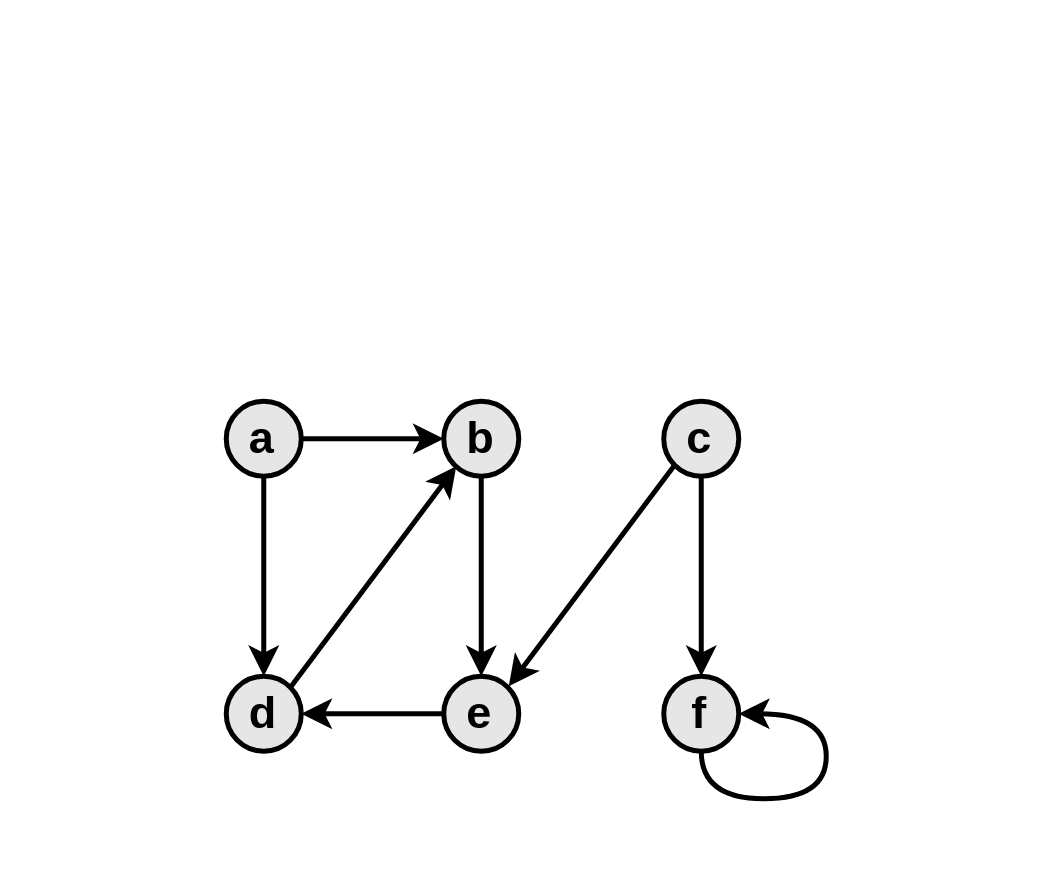
\includegraphics[width=0.5\textwidth]{pics/DirectedGraph_Alpha.png}
        \label{fig:DirectedGraph_Alpha}
    }
\centering
    \subfigure[Auxiliary vertex-label look-up index.]
    {
        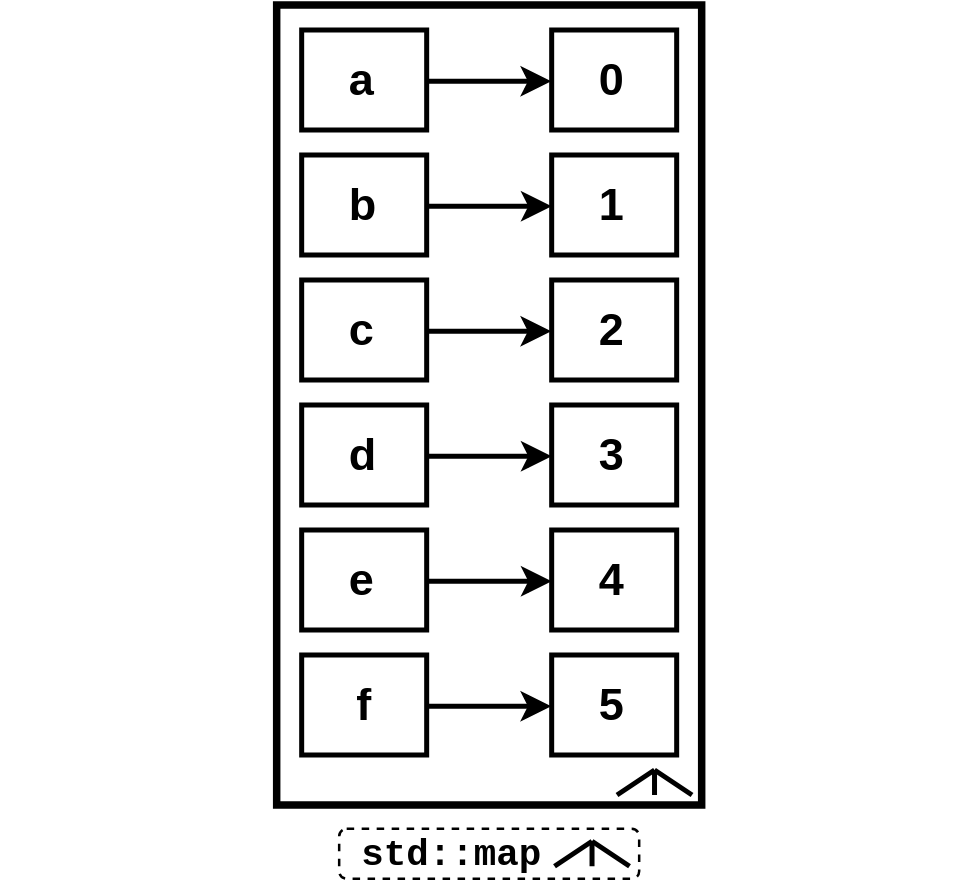
\includegraphics[width=0.4\textwidth]{pics/AdjacencyMatrix_Aux_Physical.png}
        \label{fig:AdjMat_Aux_phy}
    }
\centering
    \subfigure[Adjacency matrix physical representation of $G$.]
    {
        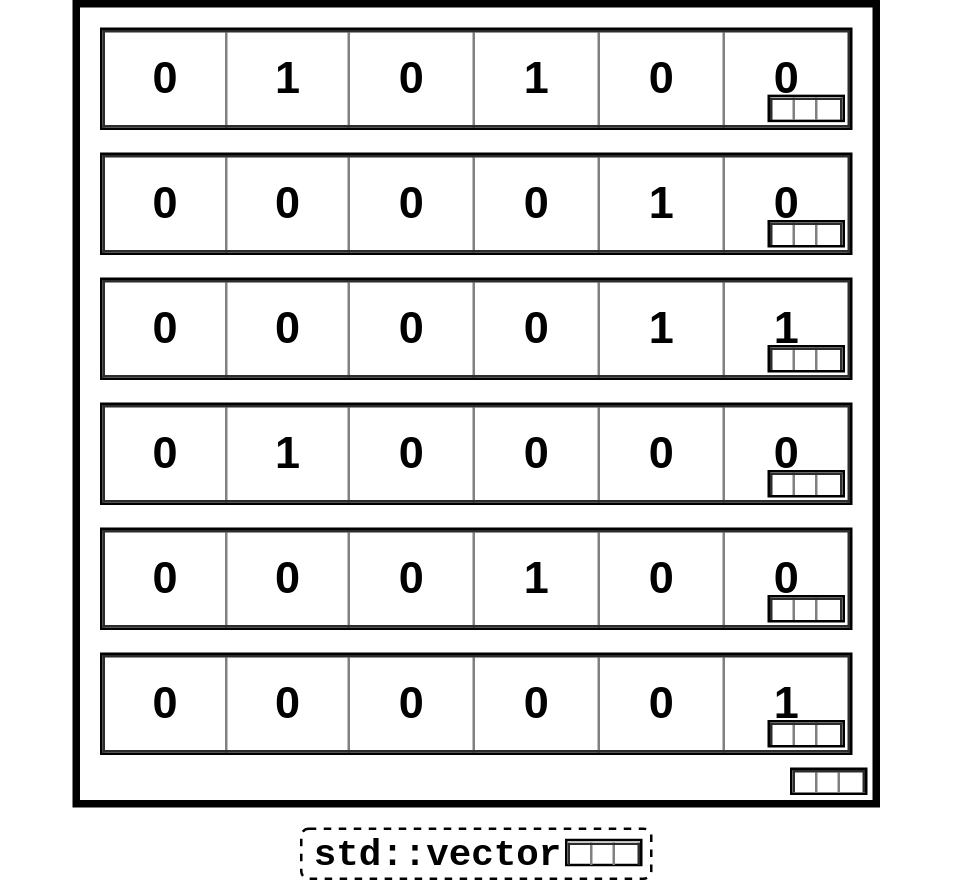
\includegraphics[width=0.42\textwidth]{pics/AdjacencyMatrix_Physical.png}
        \label{fig:AdjMat_phy}
    }
\centering
    \subfigure[CSR physical representation of $G$.]
    {
        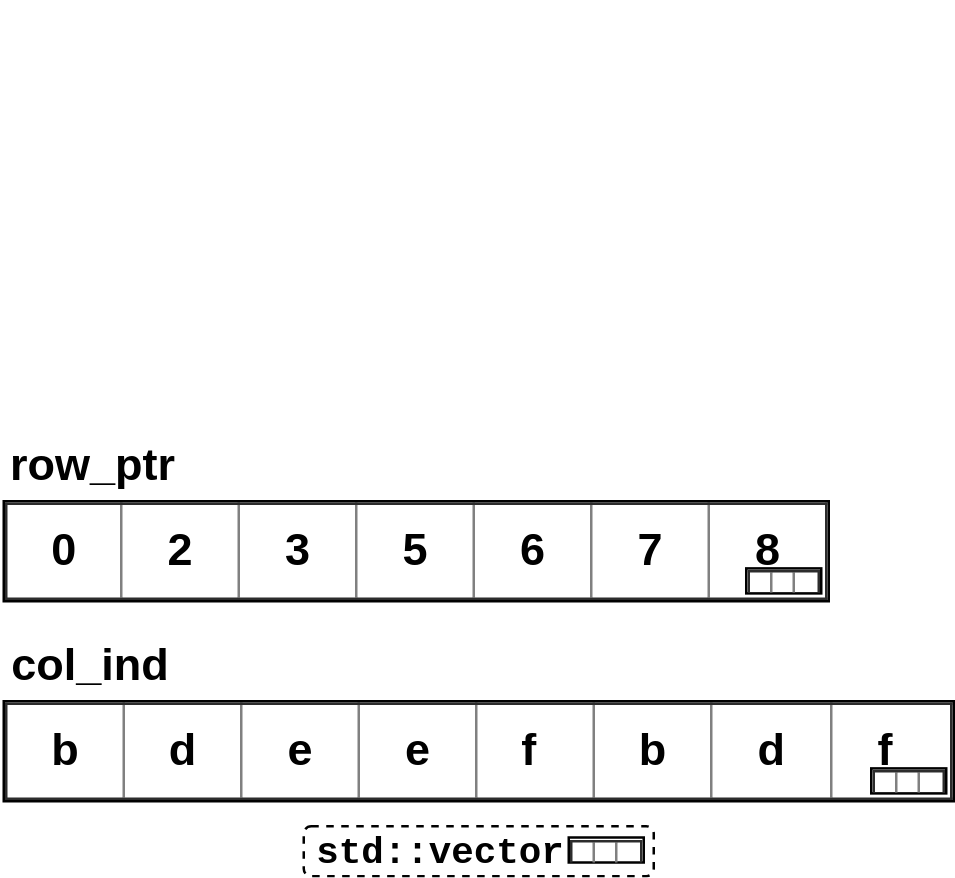
\includegraphics[width=0.4\textwidth]{pics/CSR_Physical.png}
        \label{fig:CSR_phy}
    }
\centering
    \subfigure[Adjacency list physical representation of $G$.]
    {
        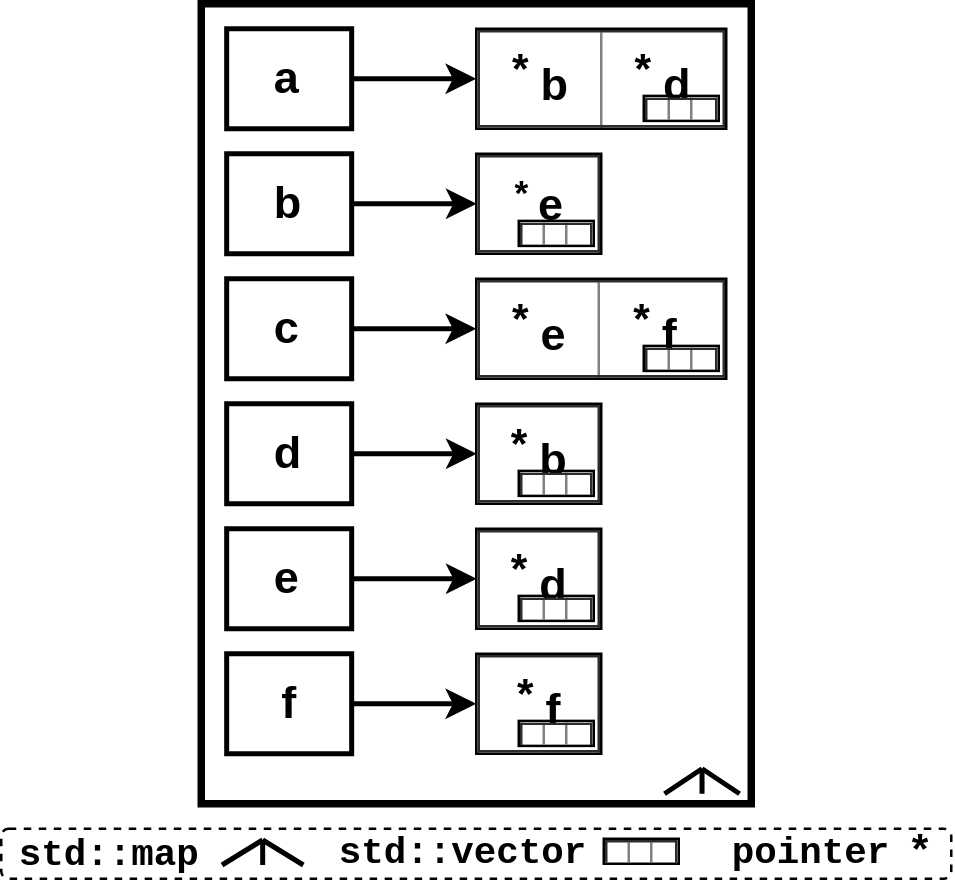
\includegraphics[width=0.4\textwidth]{pics/AdjacencyList_Physical.png}
        \label{fig:AdjLst_phy}
    }
    \caption{Physical representations of the topology of vertex-labeled directed graph \textit{G}.}
    \label{fig:GraphTopology_physical}
\end{figure}


\section{Graph Topology Structures}
\label{sec:PhyDesign-GraphTopology}

In (\ref{sec:EvalQuests}), we introduced a set of evaluation questions that we aim to answer in this thesis. In this section, we present the physical design of graph topology data structures we implemented , which we later will execute a set of evaluation tests on to find answers for the evaluation questions. We designed all the graph topology structures in this section to represent a graph that is characterized by being labeled and directed.

We used the \textit{C++} programming language in the implementation of the data structures. We utilized data structures from the $C++/STL$ library as the base for designing and implementing the graph topology data structures. We implemented all the data structures for in-memory processing of data with no involvement of disk persistent storage \cite{josuttis2012c++}.

Following, we present the physical design of three graph topology data structures (adjacency matrix, compressed sparse row (CSR), and adjacency list) in (\ref{subsec:PhyDesign-AdjacencyMatrix}, \ref{subsec:PhyDesign-CSR}, and \ref{subsec:PhyDesign-AdjacencyList}) respectively.



\subsection{Adjacency Matrix}
\label{subsec:PhyDesign-AdjacencyMatrix}

In (\ref{subsubsec:AdjacencyMatrix}), we presented the necessary background knowledge on adjacency matrices. We discussed the logical design, suitable usage scenarios, and the memory requirements of the adjacency matrix data structure. We will present in this section our physical design of adjacency matrix.

%Elements in (\texttt{std::vector}) are placed in sequence and are accessed using their index. The (\texttt{std::vector}) allocates its elements in consecutive memory locations which offers better data locality. Also, (\texttt{std::vector})'s are able to dynamically re-size to store new data. Those three characteristics have made (\texttt{std::vector}) the best choice for the design of adjacency matrix \cite{josuttis2012c++}.

We constructed the adjacency matrix physically using the (\texttt{std::vector}) data structure in $C++$. We represent each row in the adjacency matrix using a single (\texttt{std::vector}), with all of the (\texttt{std::vector})'s that represent the rows, have the same size equal to the number of vertices forming the graph. We grouped all the (\texttt{std::vector})'s that are representing the adjacency matrix rows into another (\texttt{std::vector}).

%Although the complexity of search in (\texttt{std::vector}) is $O(n)$, it provides a complexity of $O(1)$ when accessing a specific index, %which is more suitable for the use-cases where a search for the existence of an edge between two vertices is more frequent \cite{josuttis2012c++}.

In a vertex-labeled graph, each vertex is labeled with a unique label. The vertex label doesn't has to be a numeric label, however the label can be formed using a string of characters. The adjacency matrix logical design however, is assuming a numeric labeled vertices. To solve this problem, we attached an auxiliary structure to the adjacency matrix. The purpose of the auxiliary structure is to serve as a look-up index by mapping each unique vertex-label to a unique number that represents the vertex's both row-and-column index in the adjacency matrix. The auxiliary index structure is utilizing the (\texttt{std::map}) in $C++$.

%, since it provides a rich interface to manage key-value pairs. The (\texttt{std::map}) data structure is usually implemented as a binary tree providing a complexity of $O(log (n))$ on searching for an element \cite{josuttis2012c++}.

In (Figure \ref{fig:AdjMat_phy}), we show an example of the adjacency matrix physical representation of the vertex-labeled directed graph $G$ shown in (Figure \ref{fig:DirectedGraph_Alpha}). The 6x6 adjacency matrix in the figure is constructed using a set of (\texttt{std::vector})'s grouped into another (\texttt{std::vector}). In (Figure \ref{fig:AdjMat_Aux_phy}), we show the auxiliary vertex-label look-up index that maps each vertex-label in $G$ to a unique number representing the vertex's both row-and-column index in the adjacency matrix.



\subsection{Compressed Sparse Row (CSR)}
\label{subsec:PhyDesign-CSR}

In (\ref{subsubsec:CSR}), we presented the necessary background knowledge on the compressed sparse row (CSR) structure. We discussed the logical design, suitable usage scenarios, and the memory requirements of CSR. We will present in this section our physical design of the compressed sparse row (CSR).

%For constructing the compressed sparse row (CSR) we needed a data structure that is able to place elements in a sequence with access to the elements using their position, store the elements in consecutive memory locations for better data locality, and offers a dynamic size feature for accommodating new data. The (\texttt{std::vector}) data structure is matching the needed requirements and hence we choose it for the physical design of CSR. Although the complexity of search in (\texttt{std::vector}) is $O(n)$, it provides a complexity of $O(1)$ when accessing a specific index \cite{josuttis2012c++}.

%Although the complexity of search in (\texttt{std::vector}) is $O(n)$, it provides a complexity of $O(1)$ when accessing a specific index

For constructing the compressed sparse row (CSR), we utilized the (\texttt{std::vector}) data structure for the physical design of CSR. The compressed sparse row (CSR) physical design is consisted of two (\texttt{std::vector})'s. The first (\texttt{std::vector}) is representing the \textit{row\_ptr} structure and the second (\texttt{std::vector}) is representing the \textit{col\_ind} structure.

CSR inherits the same issue that adjacency matrix faces with a vertex-labeled graph, where each vertex is not limited to numeric labels but also can be labeled using a string of characters. We solve this issue in the same way we solved it in adjacency matrix by attaching an auxiliary structure to the CSR. The purpose of the auxiliary structure is to serve as a look-up index by mapping each unique vertex-label to a unique number that represents the original vertex's both row-and-column index in the adjacency matrix. As the vertex-label and the column index in the adjacency matrix are no-longer equal, we chosen to directly store the vertex-label rather than the column index in the \textit{col\_ind} structure. The auxiliary index structure is utilizing the (\texttt{std::map}) in $C++$.

%As mentioned earlier in (\ref{subsec:PhyDesign-AdjacencyMatrix}), the auxiliary index structure is utilizing the (\texttt{std::map}) in $C++$, since it provides a rich interface to manage key-value pairs. The (\texttt{std::map}) data structure is usually implemented as a binary tree providing a complexity of $O(log (n))$ on searching or insertion for an element \cite{josuttis2012c++}.

In (Figure \ref{fig:CSR_phy}), we show an example of the compressed sparse row (CSR) physical representation of the vertex-labeled directed graph $G$ shown in (Figure \ref{fig:DirectedGraph_Alpha}). The CSR physical structure in the figure is constructed using one (\texttt{std::vector}) representing the \textit{row\_ptr} structure and another (\texttt{std::vector}) representing the \textit{col\_ind} structure. In (Figure \ref{fig:AdjMat_Aux_phy}), we show the auxiliary vertex-label look-up index that maps each vertex-label in $G$ to a unique number representing the original vertex's both row-and-column index in the adjacency matrix.


\subsection{Adjacency List}
\label{subsec:PhyDesign-AdjacencyList}

In (\ref{subsubsec:AdjacencyList}), we presented the necessary background knowledge on adjacency lists. We discussed the logical design, suitable usage scenarios, and the memory requirements of the adjacency list data structure. We will present in this section our physical design of the adjacency list.

%Adjacency list logical design is storing the topology of a graph $G = (V,E)$ as a set of |$V$| pairs, where each pair is consisted of a vertex $u$ as the key and the value is a vector $K$ that contains the adjacencies of $u$. We constructed the adjacency list using the (\texttt{std::map}) data structure in $C++$. The (\texttt{std::map}) data structure provides a rich interface to manage key-value pairs. The (\texttt{std::map}) data structure is usually implemented as a binary tree providing a complexity of $O(log (n))$ on searching for an element. The underlying binary tree in (\texttt{std::map}) is providing the ability to dynamically expand with less overhead of reorganizing the elements when compared to other key-value store data structures(e.g. the static hash-table based data structures) \cite{josuttis2012c++}.

Adjacency list logical design is storing the topology of a graph $G = (V,E)$ as a set of |$V$| pairs, where each pair is consisted of a vertex $u$ as the key and the value is a vector $K$ that contains the adjacencies of $u$. We constructed the adjacency list using the (\texttt{std::map}) data structure in $C++$.

Each key-value pair ($u,K)$ in adjacency list is represented physically by a key-value pair in a (\texttt{std::map}). Each key-value pair in the (\texttt{std::map}) is consisted of an atomic value representing a unique vertex-label of a vertex $u$ mapped to a (\texttt{std::vector}) of vertex-pointers. Each vertex-pointer in a (\texttt{std::vector}) is pointing to its respective vertex key in the adjacency list (\texttt{std::map}).

%The (\texttt{std::vector}) data structure is able to place elements in a sequence with access to the elements using their position, store the elements in consecutive memory locations for better data locality, and offers a dynamic size feature for accommodating new data. Also, the (\texttt{std::vector}) data structure is usually implemented as a dynamic array providing a complexity of $O(n)$ on searching for an element and $O(1)$ on access by an element's position \cite{josuttis2012c++}.

In (Figure \ref{fig:adjLst_logical}), we show an example of the adjacency list physical representation of the vertex-labeled directed graph $G$ shown in (Figure \ref{fig:DirectedGraph_Alpha}). The adjacency list in the figure is constructed using a (\texttt{std::map}) of 6 key-value pairs. An example of a key-value pair is the second key-value pair which is consisted of the vertex-label of vertex $b$ and its adjacencies vector that contains only one pointer to the key of the fifth pair in the (\texttt{std::map}) (i.e. a pointer to vertex $f$).

\section{Graph Properties Structures}
\label{sec:PhyDesign-GraphProperties}

In (\ref{sec:PhyDesign-GraphTopology}), we presented the physical design of graph topology structures. In this section, we proceed with the introduction of our physical design for more graph data structures. we present the physical design of graph properties. We designed all the graph properties structures to support all the characteristics of the property graph model. 

We continue using the \textit{C++} programming language in the implementation of the data structures. We utilized data structures from the $C++/STL$ library as the base for designing and implementing the graph topology data structures. We implemented all the data structures for in-memory processing of data with no involvement of disk persistent storage (for more information on \textit{C++} or $STL$, see \cite{josuttis2012c++}).

We will use the attributed directed graph $G$ in (\ref{fig:PropertyGraph_physical}), to showcase an example of the physical representation of the properties describing each vertex or edge in $G$. Even though graph $G$ is attributed, it is not explicitly defining an identifying label for each object. The property $"id"$ that describes the vertices is appearing to have a unique value for each vertex and hence we used it to act as the vertex-label. For edges, we found three properties that we can use to uniquely identify each edge. The three properties are the $"id"$ property of the source vertex, the $"id"$ property of the target vertex, and the $"type"$ property of an edge. The concatenation of the three properties is acting as the edge-label.

Following, we present the physical design of the three graph properties data structures (universal table, emerging schema, and nested key-value store) in (\ref{subsec:PhyDesign-UniversalTable}, \ref{subsec:PhyDesign-EmergingSchema}, and \ref{subsec:PhyDesign-NestedStore}) respectively.




\begin{figure}[H]
\centering
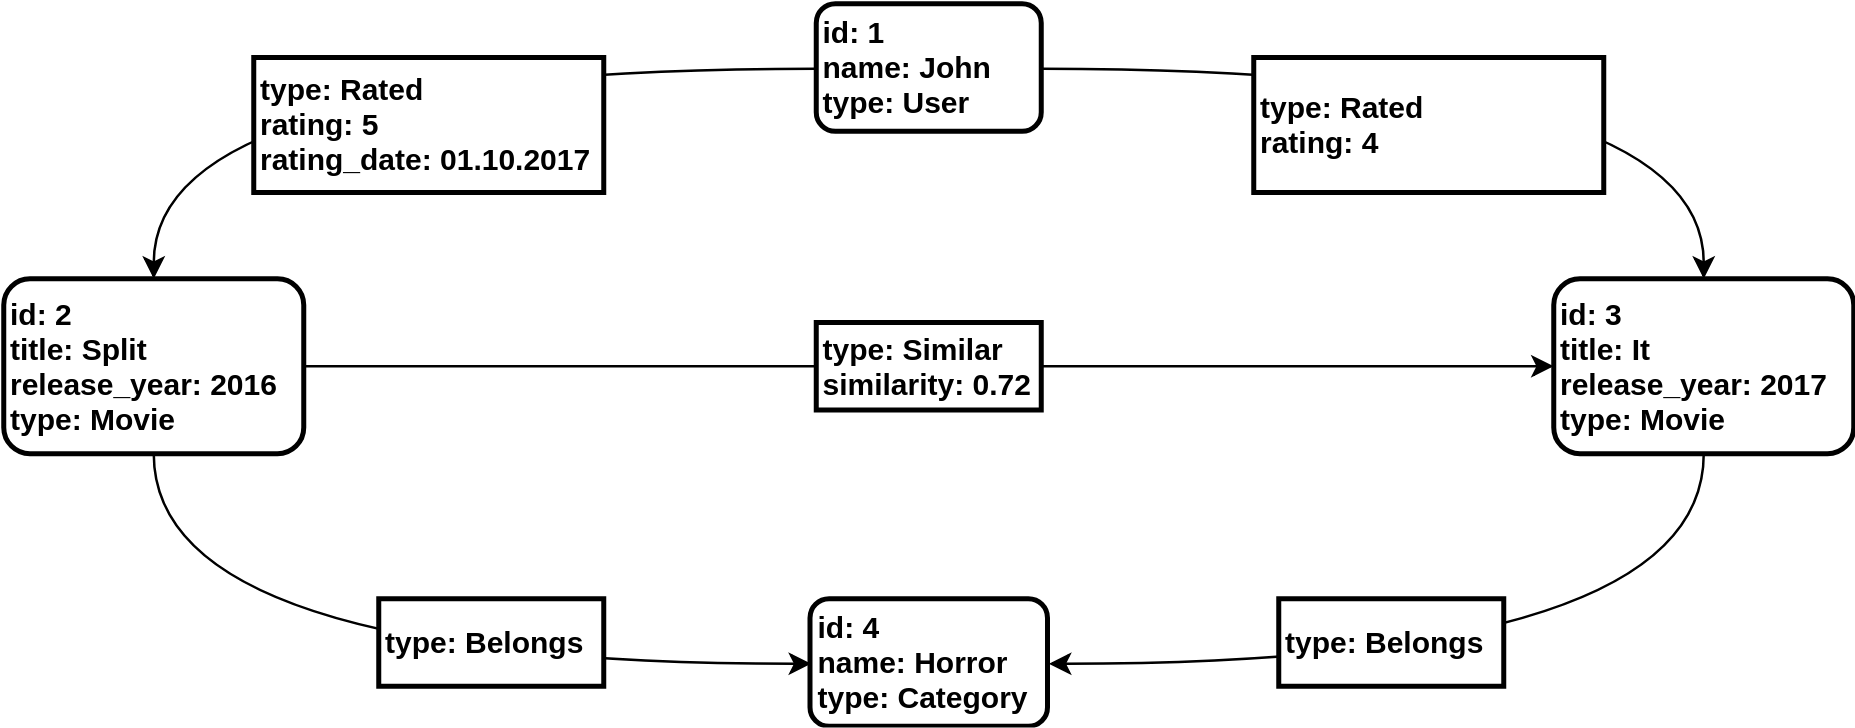
\includegraphics[width=0.9\textwidth]{pics/PropertyGraph.png}
\caption{An attributed directed graph \textit{G} \cite{DBLP:journals/corr/ParadiesLB14}.}
\label{fig:PropertyGraph_physical}
\end{figure} 






%We constructed the universal table physically using the (\texttt{std::map}) data structure in $C++$. The (\texttt{std::map}) data structure is usually implemented as a binary tree providing a complexity of $O(log (n))$ on searching for an element and hence providing fast access to a universal table's row. We represent each row in the universal table using a single key-value pair in the (\texttt{std::map}). The value(s) of the primary key column(s) of the universal table is/are used as the key in the (\texttt{std::map}), and the rest of the columns' values are placed in a (\texttt{std::vector}) representing the value of the key-value pair in the (\texttt{std::map}). If the primary key is composed of more than one column, the values are concatenated to form a single key \cite{josuttis2012c++}.

\begin{figure}[H]
\centering
    \subfigure[Vertex universal table physical representation.]
    {
        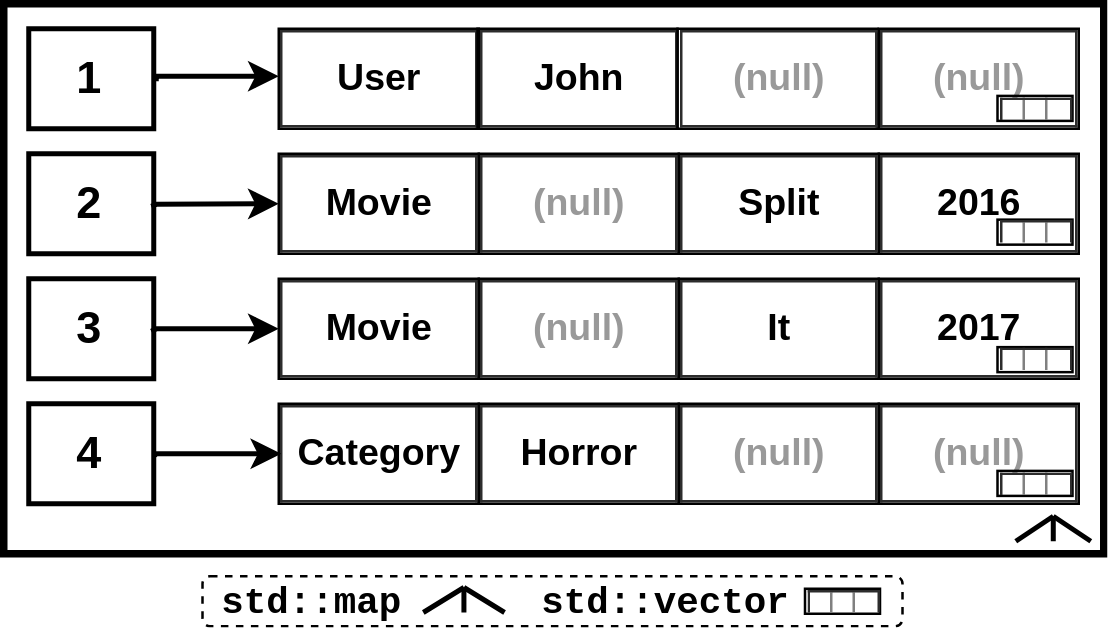
\includegraphics[width=0.57\textwidth]{pics/VertexUniversalTable_Physical.png}
        \label{fig:VertexUniTbl_physical}
    }
\centering
    \subfigure[Vertex header table.]
    {
        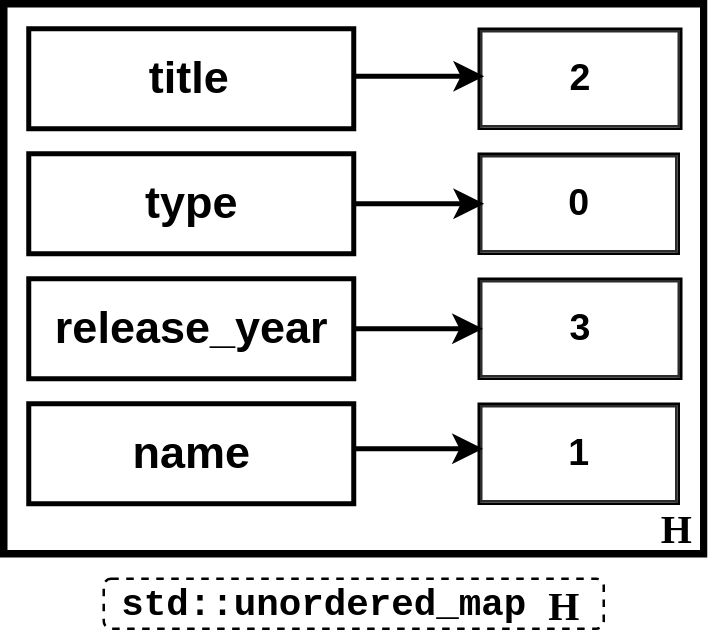
\includegraphics[width=0.362\textwidth]{pics/VertexPropertiesTable_Physical.png}
        \label{fig:VertexPropTbl_physical}
    }
\centering
    \subfigure[Edge universal table physical representation.]
    {
        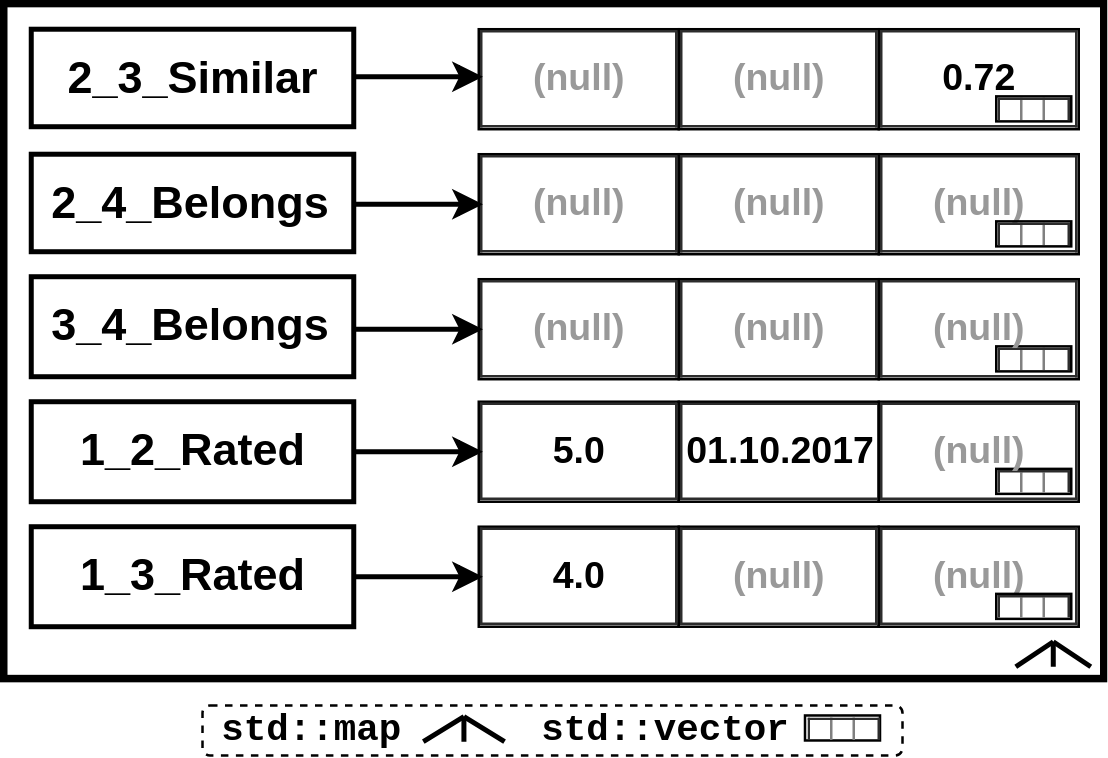
\includegraphics[width=0.57\textwidth]{pics/EdgeUniversalTable_Physical.png}
        \label{fig:EdgeUniTbl_physical}
    }
\centering
    \subfigure[Edge header table.]
    {
        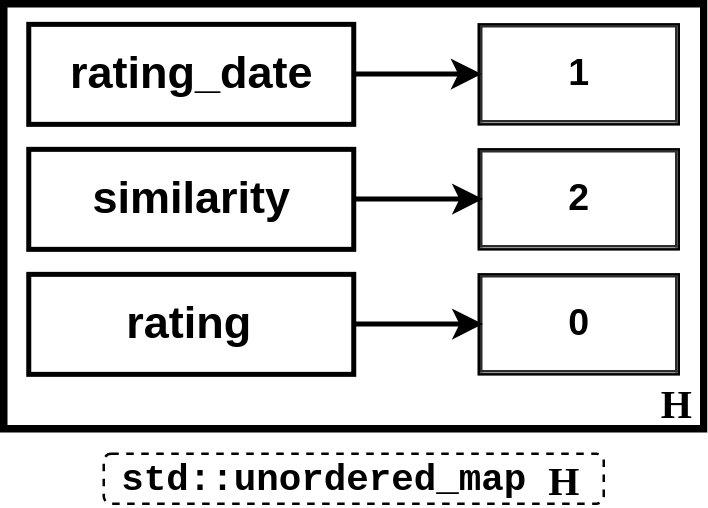
\includegraphics[width=0.36\textwidth]{pics/EdgePropertiesTable_Physical.png}
        \label{fig:EdgePropTbl_physical}
    }
    \caption{Universal table physical representation of graph \textit{G} shown in (\ref{fig:PropertyGraph_physical}).}
    \label{fig:UniversalTable_physical}
\end{figure}

\subsection{Universal Table}
\label{subsec:PhyDesign-UniversalTable}

In (\ref{subsubsec:UniversalTable}), we presented the necessary background knowledge on universal tables. We discussed the logical design, suitable usage scenarios, advantages, and disadvantages of the universal table data structure. In this section, we will present our physical design of the universal table.

We constructed the universal table physically using the (\texttt{std::map}) data structure in $C++$. We represent each row in the universal table using a single key-value pair in the (\texttt{std::map}).  We use the label of the object (vertex or edge) as the row key, and a (\texttt{std::vector}) that contains the rest of the values to represent the row value. Vertex universal table is physically represented by one (\texttt{std::map}), while the edge universal table is represented by another (\texttt{std::map}). The header of the universal table is stored in a separate data structure of type (\texttt{std::unordered\_map}), where each property name is linked to the property's index in each of the (\texttt{std::vector})'s in the respective universal table.

In (\ref{fig:UniversalTable_physical}), we show the universal table physical representation of the attributed directed graph $G$ shown in (\ref{fig:PropertyGraph_physical}). The graph $G$ is represented physically using a vertex universal table in (Figure \ref{fig:VertexUniTbl_physical}) and an edge universal table in (Figure \ref{fig:EdgeUniTbl_physical}), which are storing the values of the attributes describing the graph's vertices and edges. The header of the vertex universal table and edge universal table are stored in a vertex header table in (Figure \ref{fig:VertexPropTbl_physical}) and an edge header table in (Figure \ref{fig:EdgePropTbl_physical}) respectively. 


\subsection{Emerging Schema}
\label{subsec:PhyDesign-EmergingSchema}

In (\ref{subsubsec:EmergingSchema}), we presented the necessary background knowledge on emerging schema. We discussed the logical design, suitable usage scenarios, advantages, and disadvantages of the emerging schema data structure. In this section, we will present  our physical design of the emerging schema.

Emerging schema is consisting of a set of column groups formed by applying a clustering algorithm on the columns of the universal table, resulting in the grouping of the columns with frequent co-occurring values together into the same column group. We constructed an emerging schema column group physically using the (\texttt{std::map}) data structure in $C++$ similar to the physical design of a universal table. We represent each row of a column group using a single key-value pair in the (\texttt{std::map}). We use the label of the object (vertex or edge) as the row key, and the rest of the values are placed in a (\texttt{std::vector}) that represents the row value. If the object-label is composed of more than one column, the values are concatenated to form a single key. Next, we assign each column group a unique column-group-id. Finally, all the key-value pairs formed from the column-group-id and its respective column group are placed into a single (\texttt{std::unordered\_map}) data structure.

We used the k-means clustering algorithm to vertically partition the universal table columns into a set of column groups \cite{macqueen1967}. A Vertex emerging schema is physically represented by one (\texttt{std::unordered\_map}), while the edge emerging schema is represented by another (\texttt{std::unordered\_map}). The information concerning which column group a property belongs to, and the column index of the property inside the column group is stored in separate data structure of type (\texttt{std::unordered\_map}), where each property is linked to a pair of values comprises the property column group and the property index inside the column group respectively.

In (\ref{fig:EmergingSchema_physical}), we show the emerging schema physical representation of the attributed directed graph $G$ shown in (\ref{fig:PropertyGraph_physical}). The graph $G$ is represented physically using a vertex emerging schema in (Figure \ref{fig:VertexEmergingSchema_physical}) and an edge emerging schema in (Figure \ref{fig:EdgeEmergingSchema_physical}), which are storing the values of the properties describing the graph's vertices and edges in column groups based on their frequency of co-occurrence. The emerging schema vertex header table in (Figure \ref{fig:ESVertexPropTbl_physical}) is storing for each property, the column-group-id of the column group containing the property, followed by the property index in the respective column group. The column-group-id together with the property position are grouped into a (\texttt{std::pair}) data structure. Similarly, the emerging schema edge header table is shown in (Figure \ref{fig:ESEdgePropTbl_physical}).



\begin{figure}[H]
\centering
    \subfigure[Vertex emerging schema physical representation.]
    {
        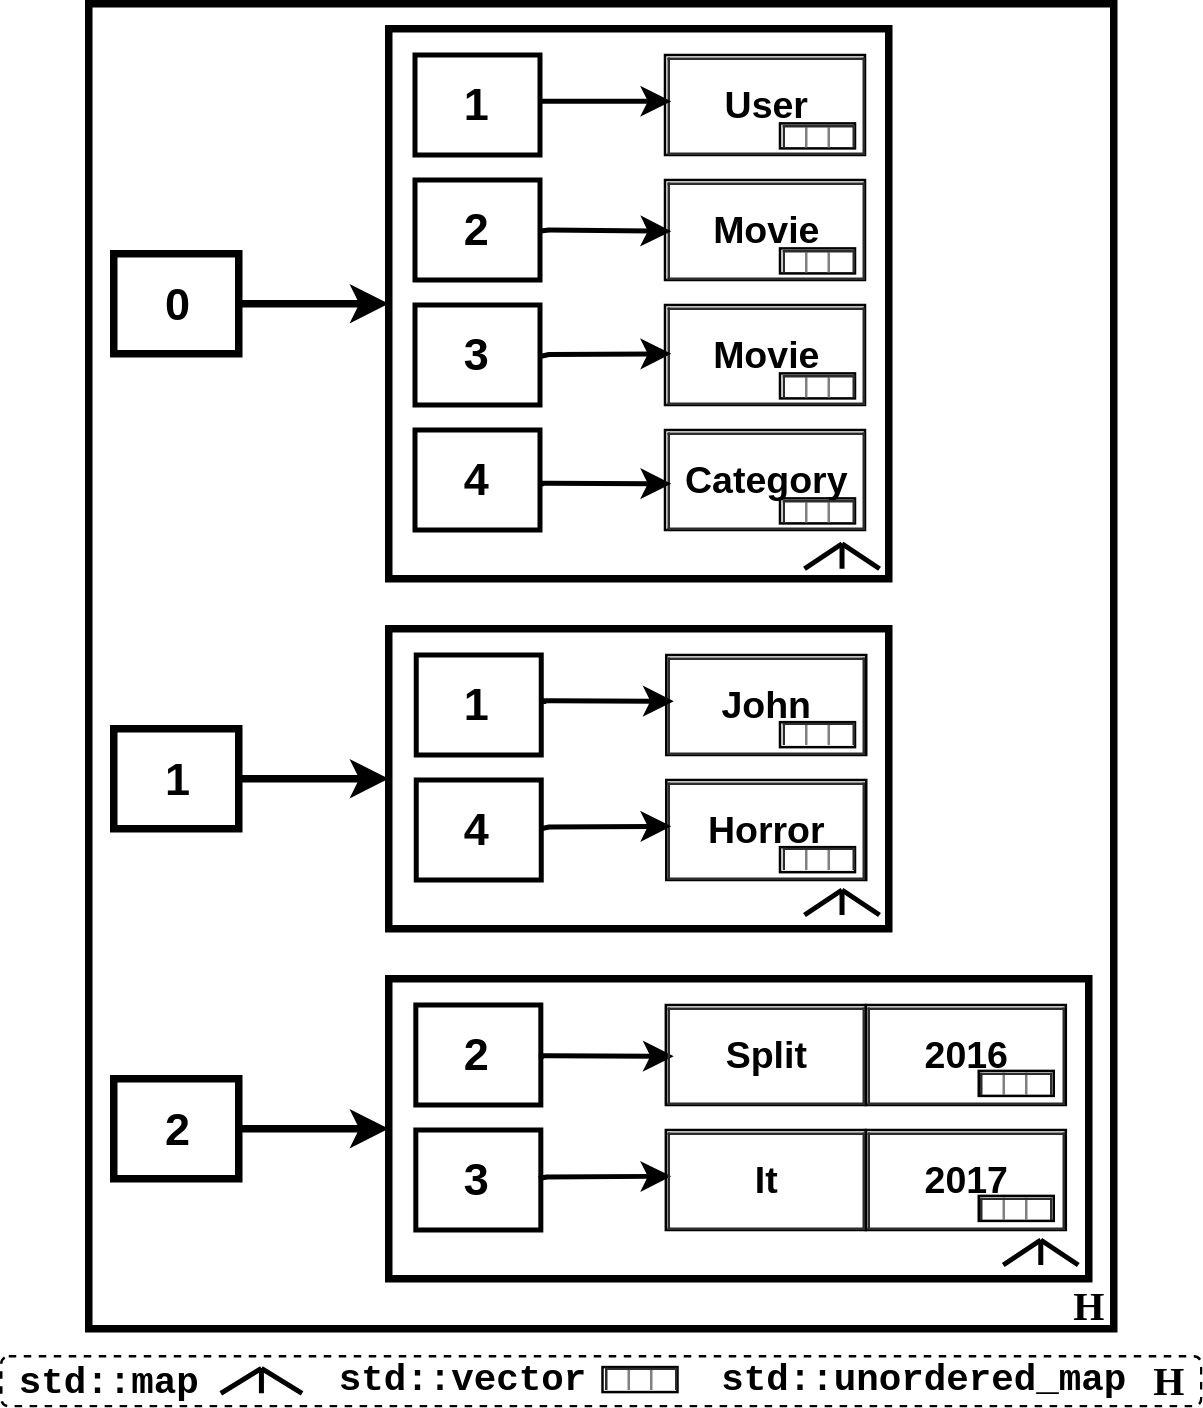
\includegraphics[width=0.58\textwidth]{pics/VertexEmergingSchema_Physical.png}
        \label{fig:VertexEmergingSchema_physical}
    }
\centering
    \subfigure[Emerging schema vertex header table.]
    {
        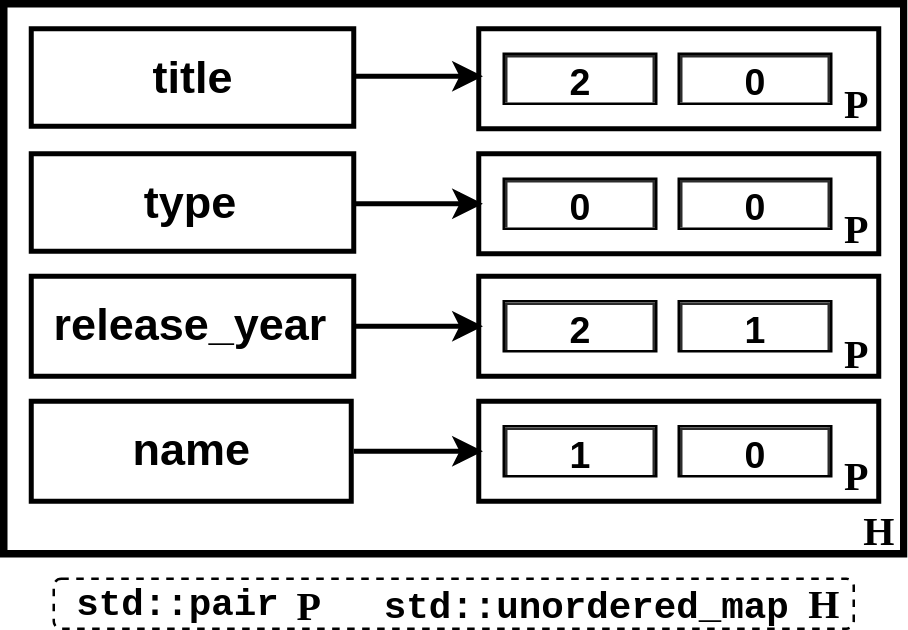
\includegraphics[width=0.37\textwidth]{pics/VertexClusteredPropertiesTable_Physical.png}
        \label{fig:ESVertexPropTbl_physical}
    }
\centering
    \subfigure[Edge emerging schema physical representation.]
    {
        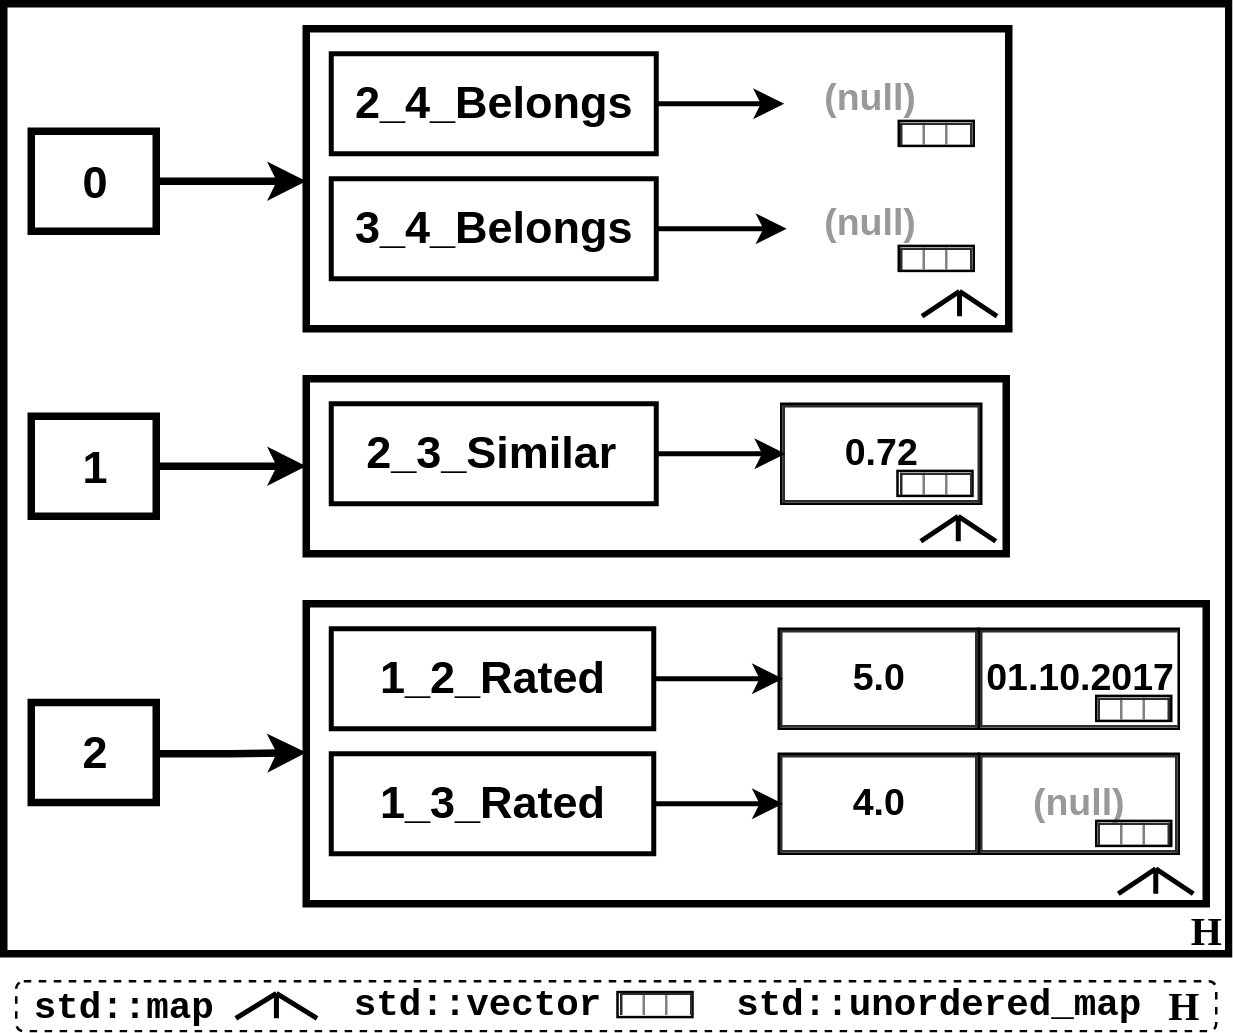
\includegraphics[width=0.58\textwidth]{pics/EdgeEmergingSchema_Physical.png}
        \label{fig:EdgeEmergingSchema_physical}
    }
\centering
    \subfigure[Emerging schema edge header table.]
    {
        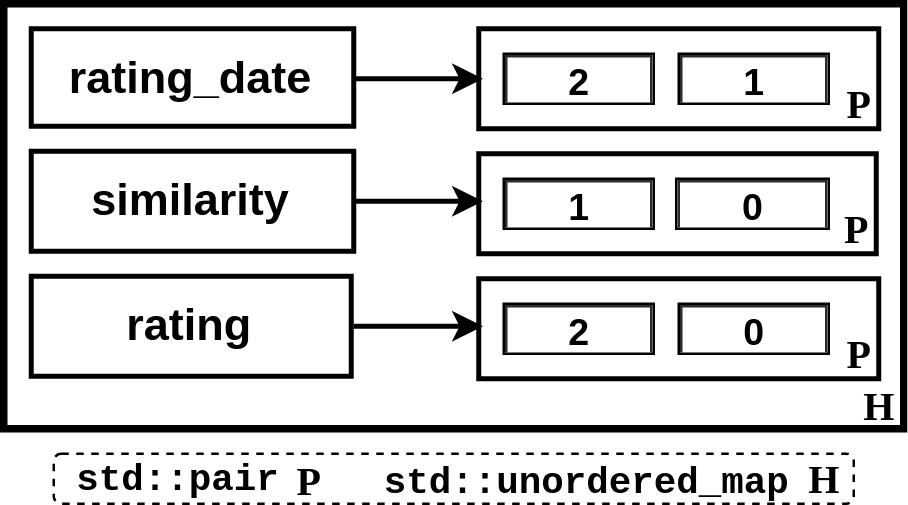
\includegraphics[width=0.37\textwidth]{pics/EdgeClusteredPropertiesTable_Physical.png}
        \label{fig:ESEdgePropTbl_physical}
    }
    \caption{Emerging schema physical representation of graph \textit{G} shown in (\ref{fig:PropertyGraph_physical}).}
    \label{fig:EmergingSchema_physical}
\end{figure}




\subsection{Nested Key-Value Store}
\label{subsec:PhyDesign-NestedStore}

In (\ref{subsubsec:NestedkeyValueStore}), we presented the necessary background knowledge on nested key-value store. We discussed the logical design, suitable usage scenarios, advantages, and disadvantages of the nested key-value store data structure. In this section, we will present our physical design of the nested key-value store.

In nested key-value stores, we store each object (vertex or edge) along with only the attributes that are applicable to this object (i.e. where a value exists). We store each object physically in the nested key-value store as a row. Each row is represented by a key-value pair, where the object-label is the row key and the row value is a container of type (\texttt{std::unordered\_map}) that contains the set of property-value pairs that describe the object. Objects with no descriptive properties are represented with a row that has an empty (\texttt{std::unordered\_map}) as a row value.

In (\ref{fig:NestedStore_physical}), we show the nested key-value store physical representation of the attributed directed graph $G$ shown in (\ref{fig:PropertyGraph_physical}). The graph $G$ is represented physically using a vertex nested key-value store in (Figure \ref{fig:VertexNestedStore_physical}) and an edge nested key-value store in (Figure \ref{fig:EdgeNestedStore_physical}), which are storing the values of the properties describing the graph's vertices and edges.

\begin{figure}[H]
\centering
    \subfigure[Vertex nested store physical representation.]
    {
        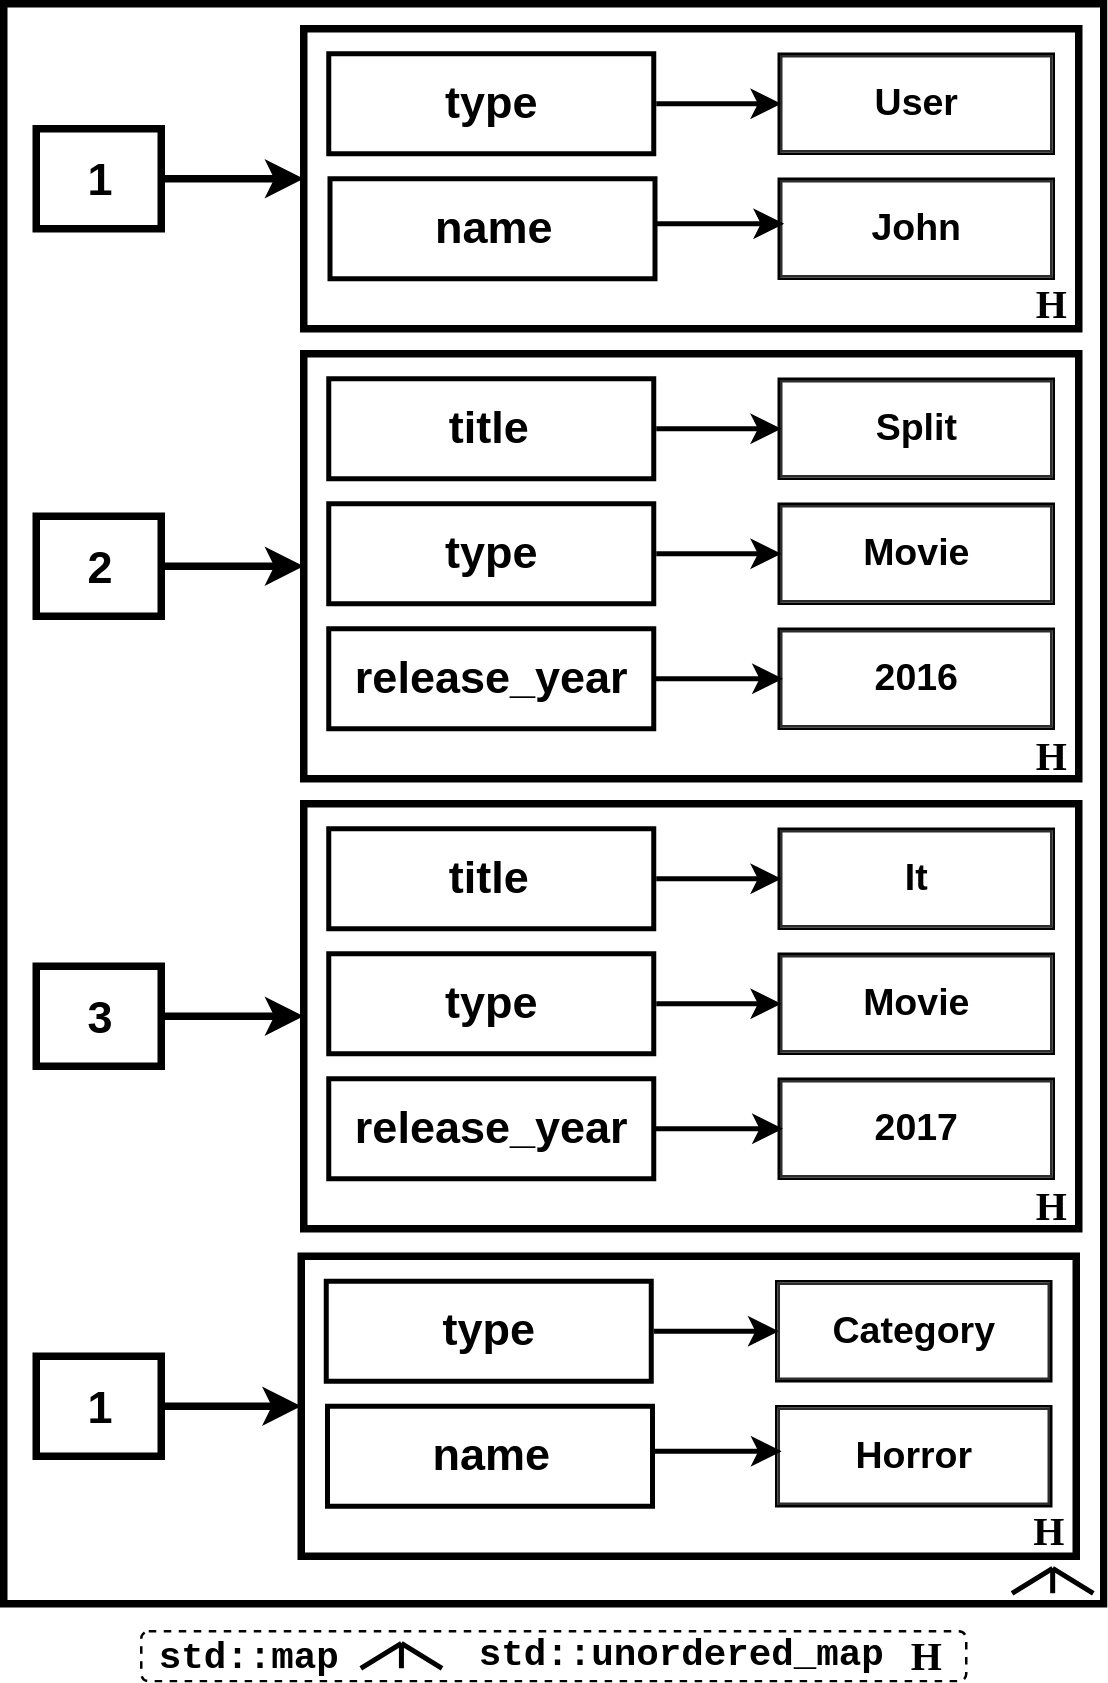
\includegraphics[width=0.45\textwidth]{pics/VertexNestedKey-ValueStore_Physical.png}
        \label{fig:VertexNestedStore_physical}
    }
\centering
    \subfigure[Edge nested store physical representation.]
    {
        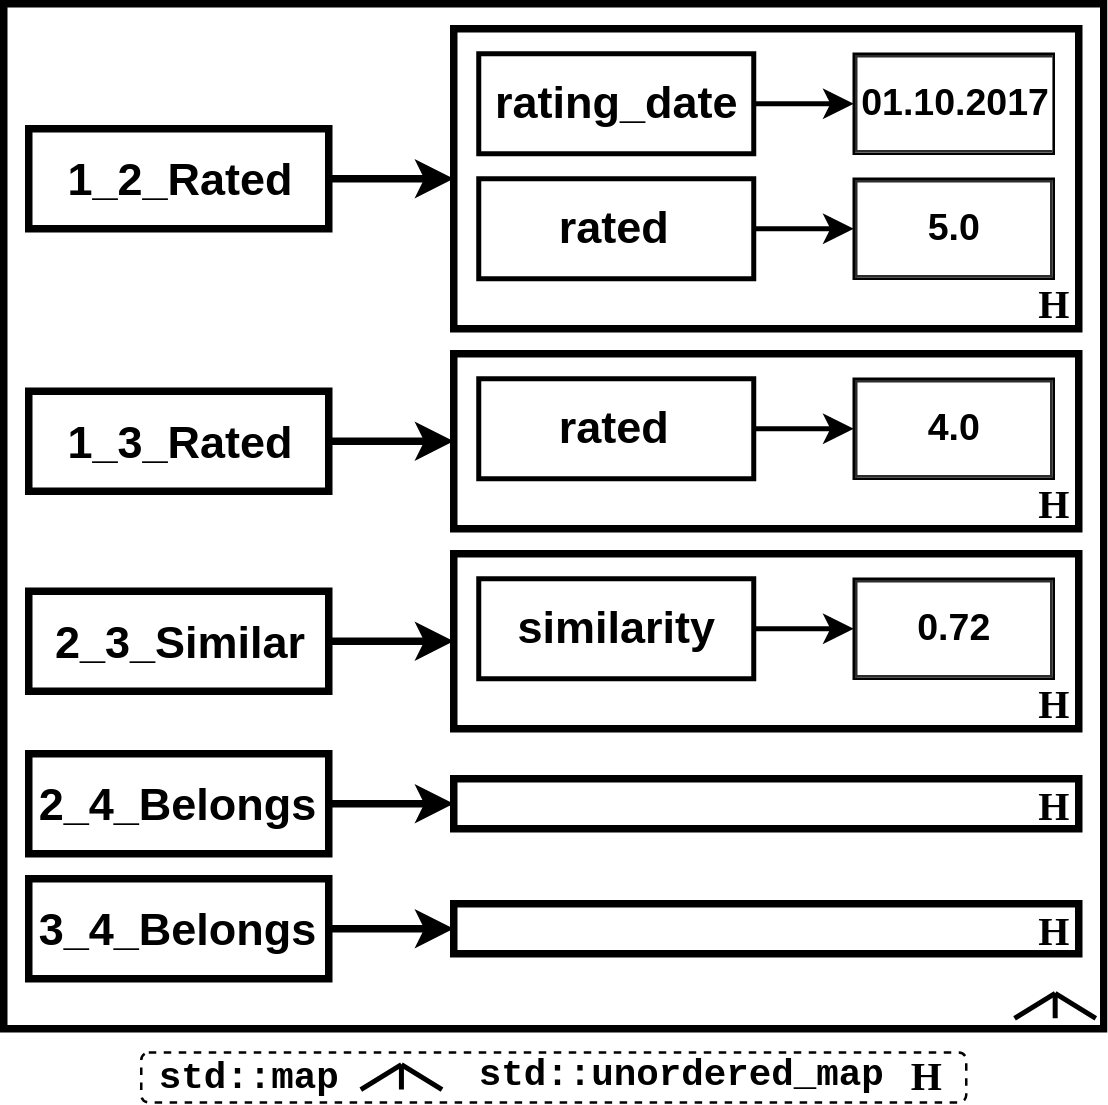
\includegraphics[width=0.45\textwidth]{pics/EdgeNestedKey-ValueStore_Physical.png}
        \label{fig:EdgeNestedStore_physical}
    }
    \caption{Nested key-value store physical representation of graph \textit{G} in (\ref{fig:PropertyGraph_physical}).}
    \label{fig:NestedStore_physical}
\end{figure}



\section{Parallel Graph Structures}
\label{sec:PhyDesign-ParallelGraphStructs}

Multiprocessor computers are offering the possibility to execute multiple instructions simultaneously with a purpose of performing computing tasks in a more efficient way \cite{cormen2009introduction}. The physical design of the graph topology data structures discussed in (\ref{sec:PhyDesign-GraphTopology}) and the graph properties data structures discussed in (\ref{sec:PhyDesign-GraphProperties}), allows for only sequential operations to be done on the data structures.

Multiple data access for read and write simultaneously can lead to a \textit{data race} problem. Data race is defined in the $C++$ standard as "two conflicting actions in different threads, at least one of which is not atomic, and neither happens before the other". To allow for parallel operations on the data structures, we used the (\texttt{std::shared\_timed\_mutex}) primitive provided in the $C++$ programming language to synchronize the access to the data structures and protect them from simultaneously being modified by multiple threads \cite{josuttis2012c++}.

The (\texttt{std::shared\_timed\_mutex}) primitive is providing the following four main functions in its interface \cite{josuttis2012c++}:
\begin{itemize}  

\item{\texttt{lock()}}\\
Locks the mutex in exclusive mood, blocks the execution if the mutex is already locked.

\item{\texttt{lock\_shared()}}\\
Locks the mutex in shared mood, blocks the execution if the mutex is already locked in exclusive mood.

\item{\texttt{unlock()}}\\
Unlocks a mutex that is currently in an exclusive lock mood.

\item{\texttt{unlock\_shared()}}\\
Unlocks a mutex that is currently in a shared lock mood.

\end{itemize}

In this section, we present a parallel version of the adjacency list data structure in (\ref{subsec:PhyDesign-ParallelAdjacencyList}) as an example of a parallel graph topology structure, as well as a parallel version of the nested key-value store in (\ref{subsubsec:NestedkeyValueStore}) as an example of a parallel graph properties structure. The parallel data structures are allowing for multiple data readers and writers performing operations concurrently making use of the (\texttt{std::shared\_timed\_mutex}) primitive to protect against a data race.



\subsection{Parallel Adjacency List}
\label{subsec:PhyDesign-ParallelAdjacencyList}

In (\ref{subsec:PhyDesign-AdjacencyList}), we discussed our physical design of adjacency list, on which we can operate only using a single thread. In this section, we extend the physical design of the adjacency list in (\ref{subsec:PhyDesign-AdjacencyList}) to support multiple threads to operate over the data structure simultaneously in parallel. We will call the adjacency list discussed in (\ref{subsec:PhyDesign-AdjacencyList}) a single thread adjacency list.

We extended the physical design of the single thread adjacency list with a global (\texttt{std::shared\_timed\_mutex}) primitive, which we use to protect the (\texttt{std::map}) of the adjacency list against concurrent writes from multiple threads.

Any thread that needs to read any data from the adjacency list (\texttt{std::map}) is required to acquire a lock on the global (\texttt{std::shared\_timed\_mutex}) in shared mood using the \texttt{lock\_shared()} function. Acquiring the lock on the (\texttt{std::shared\_timed\_mutex}) in shared mood, allows multiple threads to read data from the (\texttt{std::map}) and stops any thread from acquiring an exclusive lock on the global (\texttt{std::shared\_timed\_mutex}). 

Alternatively, a thread that needs to write any data to the adjacency list (\texttt{std::map}) is required to acquire a lock on the global (\texttt{std::shared\_timed\_mutex}) in exclusive mood using the \texttt{lock()} function to stop any other thread from reading or writing to adjacency list. 

Once a thread finishes reading or writing to the adjacency list, the thread unlocks the global (\texttt{std::shared\_timed\_mutex}) using the  \texttt{unlock()} function in case the thread has holds an exclusive lock on the mutex or using the  \texttt{unlock\_shared()} in case the thread holds a shred lock on the mutex. This allows other threads to be able to acquire lock on the mutex.

Both, the adjacency list along with the attached (\texttt{std::shared\_timed\_mutex}) allow for parallel access to the data structure by multiple threads.


\subsection{Parallel Nested Key-Value Store}
\label{subsec:PhyDesign-ParallelNestedStore}

In (\ref{subsec:PhyDesign-NestedStore}), we discussed our physical design of the nested key-value store which allows only for a single thread to operate on the data. In this section, we extend the physical design of the nested key-value store in (\ref{subsec:PhyDesign-NestedStore}) to support multiple threads to operate over the data structure simultaneously in parallel.

Similar to the extension we made to the single thread adjacency list in order to support parallel access, we extended the physical design of the single thread nested key-value store with a global (\texttt{std::shared\_timed\_mutex}) primitive, which we use to protect the (\texttt{std::map}) of the nested store against concurrent writes from multiple threads. We used one (\texttt{std::shared\_timed\_mutex}) primitive to manage the access to the vertex nested key-value store and another (\texttt{std::shared\_timed\_mutex}) primitive to mange the access to the edge nested key-value store.

Any thread that needs to read any data from the nested store (\texttt{std::map}) is required to acquire a lock on the respective (\texttt{std::shared\_timed\_mutex}) in shared mood using the \texttt{lock\_shared()} function, allowing other threads to simultaneously read data from the nested store and stops any thread from acquiring an exclusive lock on the (\texttt{std::shared\_timed\_mutex}). 
\\
Alternatively, a thread that needs to write any data to the nested store (\texttt{std::map}) is required to acquire a lock on the respective (\texttt{std::shared\_timed\_mutex}) in exclusive mood using the \texttt{lock()} function to stop any other thread from reading or writing to nested store. 

Once a thread finishes reading or writing to the nested store, the thread unlocks the respective (\texttt{std::shared\_timed\_mutex}) using the  \texttt{unlock()} function in case the thread holds an exclusive lock on the mutex or using the  \texttt{unlock\_shared()} in case the thread holds a shred lock on the mutex.

Using the nested key-value store along with the appropriate lock on the attached (\texttt{std::shared\_timed\_mutex}), allows multiple threads to access the data structure in parallel.


\section{Partitioned Graph Topology}
\label{sec:PhyDesign-GraphPartitioning}

In (\ref{sec:PhyDesign-GraphProperties}), we presented the physical design of three graph properties structures. The physical design of the graph properties structures allows for the storage of a graph that is in the form of a property graph model (i.e. directed, labeled, attributed, and multi-graph). In (\ref{sec:PhyDesign-GraphTopology}), we presented the physical design of three graph topology structures which allows for the storage of a directed and labeled graph. For consistency of the physical design between the graph topology and graph properties structures, we present in this section a method to extend the physical design of the graph topology structures to support the storage of a multi-graph.

We introduce a graph partitioning technique as an extension to the physical design of the graph topology structures. In a multi-graph multiple edges could exist between the same two vertices, where edge is identified by an edge-label assigned to it. We use the edge label assigned to each edge in the graph as the partitioning key. In a partitioned graph topology each edge-label is linked to a graph topology structure and together they offer the storage of a multi-graph. \\\\

\begin{figure}[H]
\centering
    \subfigure[A directed labeled multi-graph $G$.]
    {
        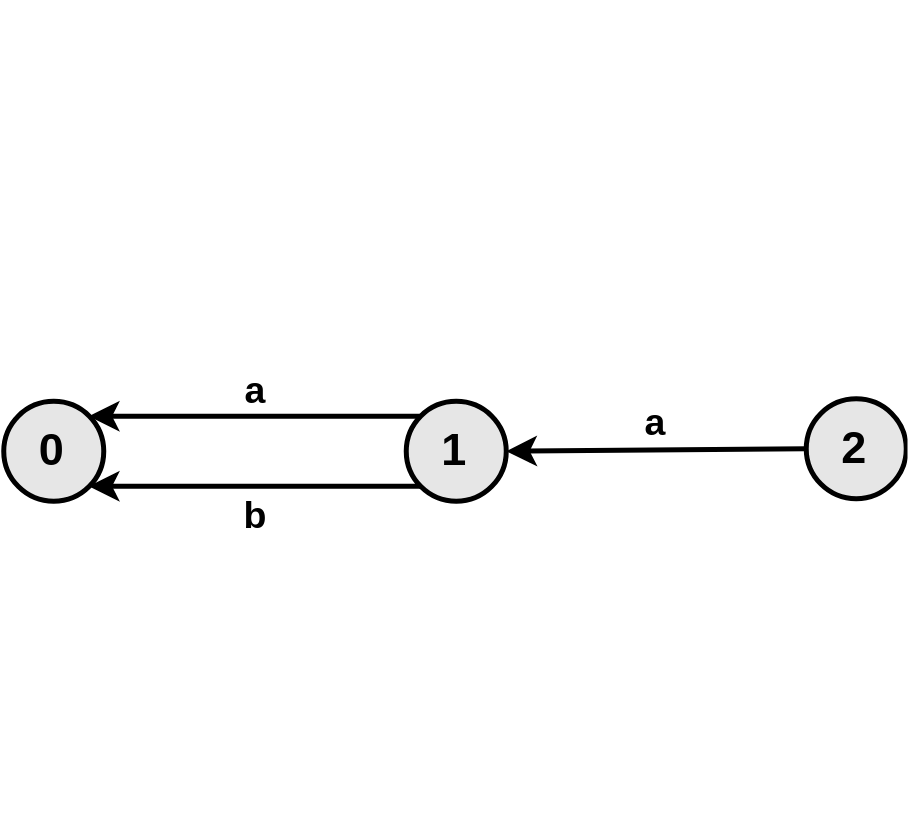
\includegraphics[width=0.40\textwidth]{pics/GraphPartitioning_graph.png}
        \label{fig:GraphPartitioning_graph}
    }
\centering
    \subfigure[Partitioned adjacency list physical representation.]
    {
        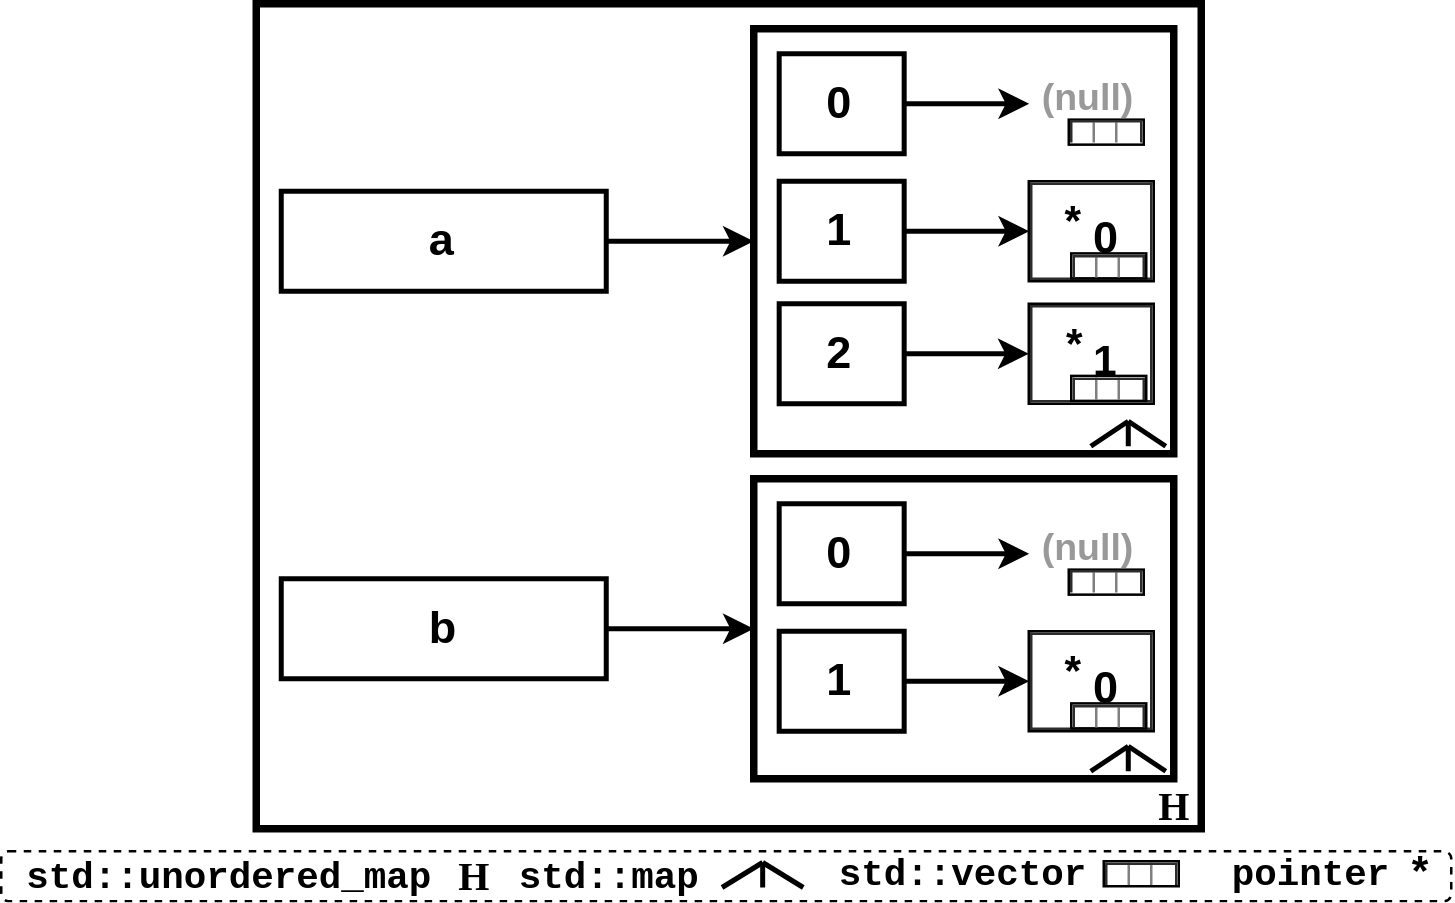
\includegraphics[width=0.55\textwidth]{pics/GraphPartitioning_physical.png}
        \label{fig:PartitionedAdjLst_physical}
    }
    \caption{Physical representation of a partitioned adjacency list of graph $G$.}
    \label{fig:GraphPartitioning_physical}
\end{figure}


We designed the partitioning technique physically using a (\texttt{std::unordered\_map}) data structure. The (\texttt{std::unordered\_map}) is storing a set of key-value pairs, where the key is an edge-label and the value is a graph topology structure. A graph topology structure that is linked to an edge-label "$x$" is storing information regarding only the vertices with at least one incoming or outgoing edge labeled with "$x$".

In (\ref{fig:GraphPartitioning_physical}), we show an example of a physical representation of a partitioned graph topology structure. We present in (Figure \ref{fig:PartitionedAdjLst_physical}) the partitioned adjacency list physical representation of the directed labeled multi-graph $G$ shown in (Figure \ref{fig:GraphPartitioning_graph}).




\section{Summary}
\label{sec:PhyDesign-Summary}

In this chapter, we presented a set of evaluation question that are focusing on evaluating the performance of graph data structures in different usage scenarios. We introduced our physical design for the graph topology structures as well as the graph properties structures. We presented a parallel version of the adjacency list and the nested key-value store structures as an example of parallel graph structures that allows for parallel access by multiple threads. We presented an extension to the physical design of the graph topology structures that allows the structures to store a multi-graph.

In next chapter, we present the evaluation environment we used to evaluate our implementation for the different graph structures.


}